\begin{figure}[htb] 
    \centering
    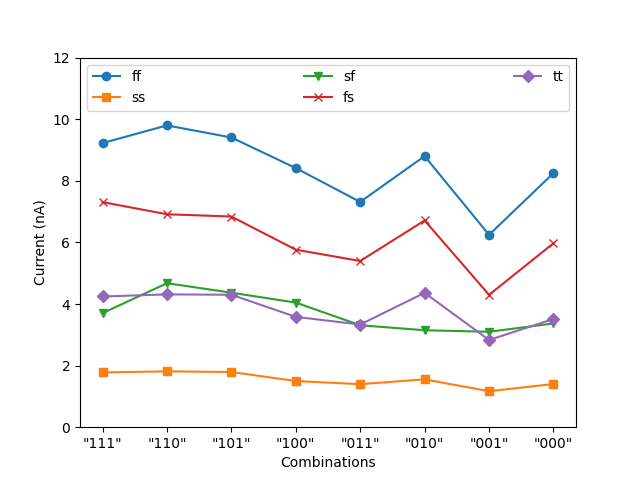
\includegraphics[width=1\textwidth]{Images/Plots/Python/baseline0.png} 
    \caption{Showing the inputs and outputs of the 0 degress baseline design.} 
    \label{fig:python0baseline} 
\end{figure}
\begin{figure}[htb] 
    \centering
    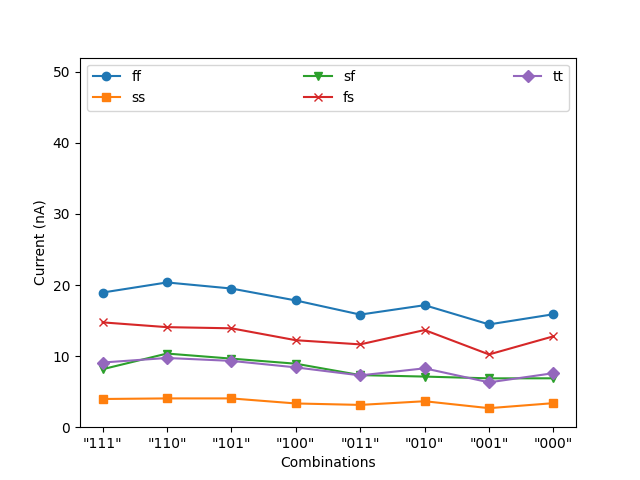
\includegraphics[width=1\textwidth]{Images/Plots/Python/baseline27.png} 
    \caption{Showing the inputs and outputs of the 27 degress baseline design.} 
    \label{fig:python27baseline} 
\end{figure}
\begin{figure}[htb] 
    \centering
    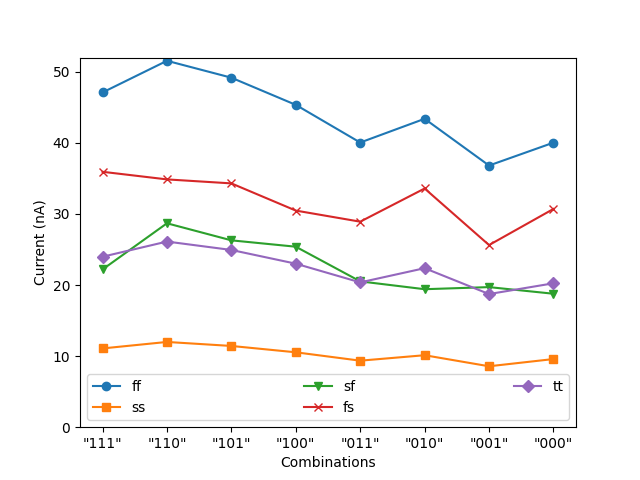
\includegraphics[width=1\textwidth]{Images/Plots/Python/baseline70.png} 
    \caption{Showing the inputs and outputs of the 70 degress baseline design.} 
    \label{fig:python70baseline} 
\end{figure}
\begin{figure}[htb] 
    \centering
    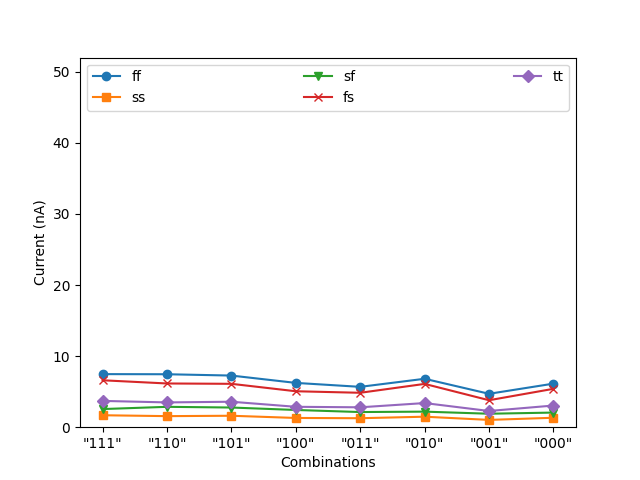
\includegraphics[width=1\textwidth]{Images/Plots/Python/improvedwl0.png} 
    \caption{Showing the inputs and outputs of the 0 degress improvedwl design.} 
    \label{fig:python0improvedwl} 
\end{figure}
\begin{figure}[htb] 
    \centering
    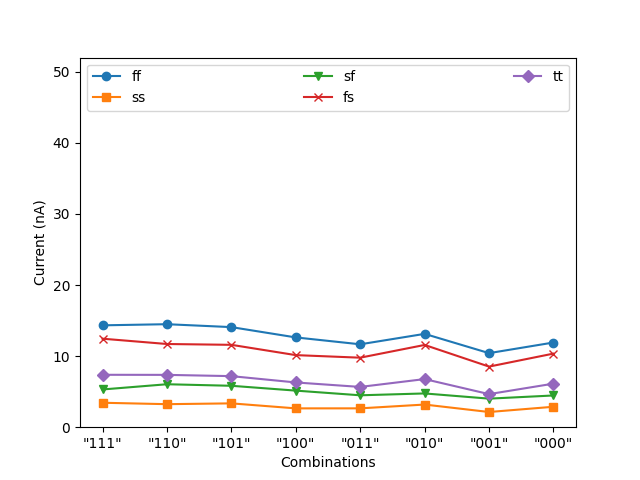
\includegraphics[width=1\textwidth]{Images/Plots/Python/improvedwl27.png} 
    \caption{Showing the inputs and outputs of the 27 degress improvedwl design.} 
    \label{fig:python27improvedwl} 
\end{figure}
\begin{figure}[htb] 
    \centering
    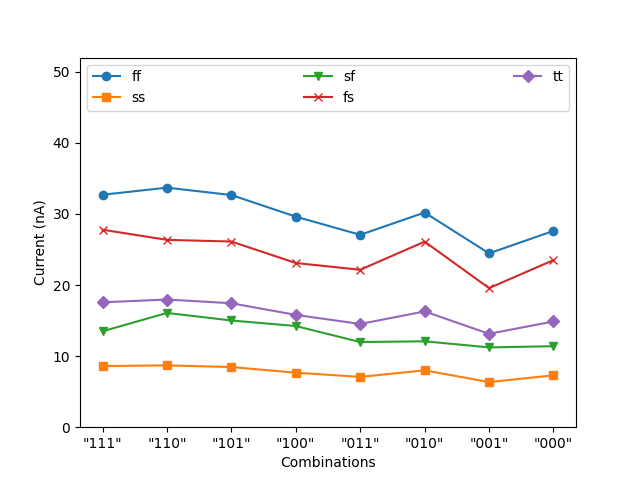
\includegraphics[width=1\textwidth]{Images/Plots/Python/improvedwl70.png} 
    \caption{Showing the inputs and outputs of the 70 degress improvedwl design.} 
    \label{fig:python70improvedwl} 
\end{figure}
\begin{figure}[htb] 
    \centering
    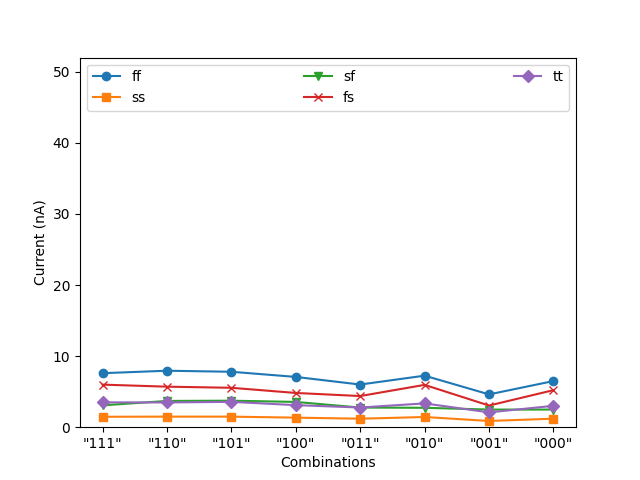
\includegraphics[width=1\textwidth]{Images/Plots/Python/reducetrans0.png} 
    \caption{Showing the inputs and outputs of the 0 degress reducetrans design.} 
    \label{fig:python0reducetrans} 
\end{figure}
\begin{figure}[htb] 
    \centering
    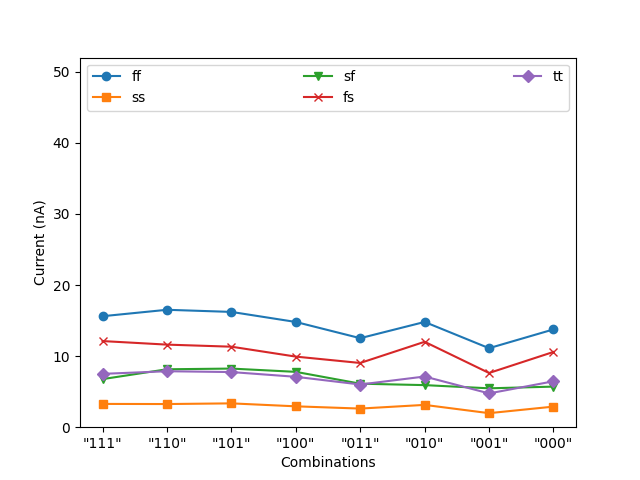
\includegraphics[width=1\textwidth]{Images/Plots/Python/reducetrans27.png} 
    \caption{Showing the inputs and outputs of the 27 degress reducetrans design.} 
    \label{fig:python27reducetrans} 
\end{figure}
\begin{figure}[htb] 
    \centering
    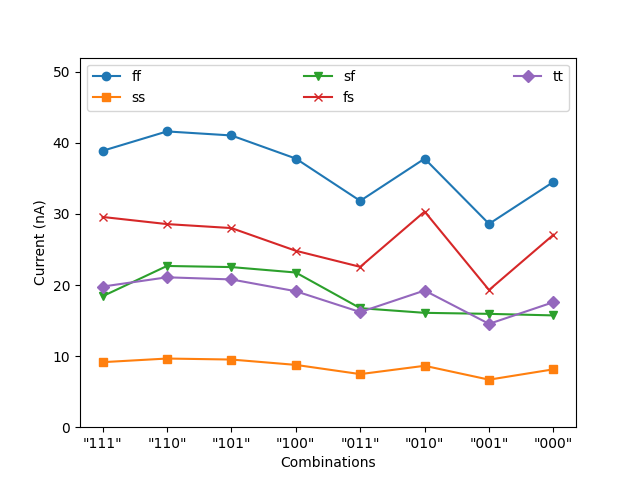
\includegraphics[width=1\textwidth]{Images/Plots/Python/reducetrans70.png} 
    \caption{Showing the inputs and outputs of the 70 degress reducetrans design.} 
    \label{fig:python70reducetrans} 
\end{figure}
\begin{figure}[htb] 
    \centering
    \includegraphics[width=1\textwidth]{Images/Plots/Python/Best0.png} 
    \caption{Showing the inputs and outputs of the 0 degress Best design.} 
    \label{fig:python0Best} 
\end{figure}
\begin{figure}[htb] 
    \centering
    \includegraphics[width=1\textwidth]{Images/Plots/Python/Best27.png} 
    \caption{Showing the inputs and outputs of the 27 degress Best design.} 
    \label{fig:python27Best} 
\end{figure}
\begin{figure}[htb] 
    \centering
    \includegraphics[width=1\textwidth]{Images/Plots/Python/Best70.png} 
    \caption{Showing the inputs and outputs of the 70 degress Best design.} 
    \label{fig:python70Best} 
\end{figure}
